\documentclass[11pt, article]{article}
\usepackage{a4wide}
\usepackage[english]{babel}
\usepackage{graphicx}
\usepackage{tabu}
\usepackage{textcomp}
\usepackage{fancyhdr}
\usepackage{lastpage}
\usepackage{titlesec}
\usepackage{lscape}
\usepackage{multicol}
\usepackage[export]{adjustbox}
\usepackage{listings}

%%%%%%
%% Variables for version and release status
%% useage: \version
%%%%%%
\newcommand\version{Max Atkins - 130017927}
\newcommand\release{CS27020}
\newcommand\titleText{Llandwp Sports}
\newcommand\reference{SE.QA.11}

%%%%%%
%% Alias
%%%%%%
\newcommand{\sectionbreak}{\clearpage} 	%% Allways start a section on a new page

\title{ \huge CS27020 Modeling Persistent Data\\ \Large \titleText}
\author{
	\vspace{100pt}
	\begin{tabular}{ r || l }
		Author 	& Max Atkins \\
						& \\
		Date Published  & \today \\
						& \\
		Department		& Computer Science \\
						&\\
		Address			& Aberystwyth University \\
						& Penglais Campas \\
						& Ceredigion \\
						& SY23 3DB \\
	\end{tabular} \\
	Copyright \textcopyright Aberystwyth University 2014
	%get rid of the date on the titlepage
	\date{}
}

\pagestyle{fancy}
\fancyhf{}
\rhead{\version}
\lhead{\release}
\rfoot{Page \thepage \hspace{1pt} of \pageref{LastPage}}
\lfoot{Aberystwyth University - Computer Science}

\begin{document}
	\setcounter{page}{1}

	\maketitle

	\tableofcontents

	\section{Normalizing the Team Card}
		%%\input{foo/bar.tex}
		
	\subsection{Keys}
	
	\underline{Primary Key} \\ \\
	\textit{Candidate Key} \\ \\
	Foreign Key* \\ \\
	
	\subsection{Un-Normalized}
	
	To create my un-normalized forms for the Team Card, I analyzed the it to identify all possible attributes, primary keys and repeating groups of attributes. I found that TeamName was an ideal Candidate key, but was not, in itself, enough to identify a team since two teams with the same name can play separate sports. 

To solve this issue, combining TeamName and SportName into a composite primary key will ensure that TeamName and SportName are unique, but there can be multiple TeamNames.

I also identified candidate keys as potentials for unique identification for other tables: CaptainID, PlayerID and TrainingID. CaptainID and PlayerID appear to be very similar, however and will be dealt with later.

When looking for functional dependencies, I realized that TrainingDay and TrainingTime would require a unique ID to be assigned to a team.

 I identified all attributes and found two repeating groups: Players and Trainings. This gave me this un-normalized form:

\begin{tabbing}
Teams( \newline \\
	\hspace{5mm}  \underline{TeamName}\\
	\hspace{5mm} \underline{SportName} \\
	\hspace{5mm} \textit{CaptainID}                      \\
	\hspace{5mm} CaptainName                 \\
	\hspace{5mm} CaptainPhone                \\
	\hspace{5mm} \textit{PlayerID}                       \\
	\hspace{5mm} PlayerName                    \\
	\hspace{5mm} \textit{TrainingID}                       \\
	\hspace{5mm} TrainingDay                     \\
	\hspace{5mm} TrainingTime                    \\
)\\
(PlayerID, PlayerName) Repeat for each team \\
(TrainingID, TrainingDay, TrainingTime) Repeat for each team
\end{tabbing}
 \newpage
 \subsection{Functional Dependencies}
To identify the functional dependencies, I analyzed the attributes to identify which unique values would depend on others. I identified the following functional dependencies: \newline \newline
TeamName and SportName, together, determine the Captain information, as these are the only attributes unique to a team. TeamName and SportName are grouped together, as specified above.\\
\textbf{(TeamName, SportName) -\textgreater (CaptainID, CaptainName, CaptainPhone)} \newline \\
CaptainID determines Captain Information, but is also determined in the above functional dependency. This creates a transitive dependency and must be dealt with later. A Captain can not be uniquely identified by their name or phone number, but can be identified by a unique ID, hence the following dependency. \\
\textbf{(CaptainID) -\textgreater (CaptainName, CaptainPhone)} \newline \\
A Player can not be uniquely determined by their name, but they can be determined by their ID number.  \\
\textbf{(PlayerID) -\textgreater (PlayerName)} \newline \\
TrainingDay and TrainingTime do not determine each other. However, I felt that a dependency was necessary to exist here to create an efficient table. To solve this, I created the TrainingID attribute, creating a TimeSlot concept to determine a combination of TrainingDay and TrainingTime. \\ 
\textbf{(TrainingID) -\textgreater  (TrainingDay, TrainingTime)} \newline \\
\newpage
\subsection{1st Normal Form}

Proceeding to 1st normal form involves splitting off the repeating groups of attributes into their own tables. This involved creating foreign keys and identifying new primary keys for each new table. Since PlayerID determines PlayerName, it becomes the primary key for the Players table and since TrainingID determines TrainingDay and TrainingTime, that becomes the primary key for the TimeSlot table. I identified the following tables:


\begin{tabbing}
Teams( \newline \\
	\hspace{5mm}  \underline{TeamName}\\
	\hspace{5mm} \underline{SportName} \\
	\hspace{5mm} CaptainID                      \\
	\hspace{5mm} CaptainName                 \\
	\hspace{5mm} CaptainPhone                \\
)\\
\\
Players( \newline \\
	\hspace{5mm}  \underline{PlayerID}\\
	\hspace{5mm} PlayerName                      \\
	\hspace{5mm}  TeamName*\\
	\hspace{5mm} SportName* \\
)\\
\\
TimeSlot( \newline \\
	\hspace{5mm}  \underline{TrainingID}\\
	\hspace{5mm} TrainingDay                     \\
	\hspace{5mm} TrainingTime \\
	\hspace{5mm}  TeamName*\\
	\hspace{5mm} SportName* \\
)\\
\end{tabbing}
\newpage
\subsection{2nd Normal Form}

Proceeding to 2nd normal form involves splitting off the partial dependencies. This involves creating a linking table between Teams and Players, since they are a many-to-many relationship (*..*). Since TimeSlot and Teams are a one-to-many relationship (a team has many timeslots, but a timeslot has one team), a direct relationship is enough and the table was unchanged from 1st normalisation.

At this stage, I also notice that, to ensure a player is unique with their team, all three attributes in the linking table must be a composite primary key.

I identified the following tables:

\begin{tabbing}
Teams( \newline \\
	\hspace{5mm}  \underline{TeamName}\\
	\hspace{5mm} \underline{SportName} \\
	\hspace{5mm} CaptainID                      \\
	\hspace{5mm} CaptainName                 \\
	\hspace{5mm} CaptainPhone                \\
)\\
\\
HasPlayers(\\
	\hspace{5mm}  \underline{TeamName*}\\
	\hspace{5mm} \underline{SportName*} \\
	\hspace{5mm}  \underline{PlayerID*}\\
)\\
\\
	
Players( \newline \\
	\hspace{5mm}  \underline{PlayerID}\\
	\hspace{5mm} PlayerName                      \\
)\\
\\
TimeSlot( \newline \\
	\hspace{5mm}  \underline{TrainingID}\\
	\hspace{5mm} TrainingDay                     \\
	\hspace{5mm} TrainingTime \\
	\hspace{5mm}  TeamName*\\
	\hspace{5mm} SportName* \\
)\\

\end{tabbing}

\newpage
\subsection{3rd Normal Form}

Proceeding to 3rd normal form involves splitting off transitive dependencies. I only have one of these, and since a Captain is essentially a Player, the CaptainID can be linked directly to the Players table to retrieve a single player. 

I identified the following tables:

\begin{tabbing}
Teams( \newline \\
	\hspace{5mm}  \underline{TeamName}\\
	\hspace{5mm} \underline{SportName} \\
	\hspace{5mm} CaptainID*                     \\
)\\
\\
HasPlayers(\\
	\hspace{5mm}  \underline{TeamName*}\\
	\hspace{5mm} \underline{SportName*} \\
	\hspace{5mm}  \underline{PlayerID*}\\
)\\
\\
	
Players( \newline \\
	\hspace{5mm}  \underline{PlayerID}\\
	\hspace{5mm} PlayerName                      \\
)\\
\\
TimeSlot( \newline \\
	\hspace{5mm}  \underline{TrainingID}\\
	\hspace{5mm} TrainingDay                     \\
	\hspace{5mm} TrainingTime \\
	\hspace{5mm}  TeamName*\\
	\hspace{5mm} SportName* \\
)\\

\end{tabbing}

	\section{Normalizing the Member Card}
		%%\input{foo/bar.tex}

\subsection{Un-Normalized}
	
	To create my un-normalized forms for the Member Card, I followed the same steps as used for the previous card. I identified a more complicated set of repeating attributes, however. Each Member has a repeating SportName attribute, and for each repeating SportName, a repeating TeamName occurs. This nested repeating group needs to be split in turn from the inside out.

This gave me this un-normalized form:

\begin{tabbing}
Teams( \newline \\
	\hspace{5mm}  \underline{MemberNumber}\\
	\hspace{5mm} MemberName                 \\
	\hspace{5mm} MemberPhone                \\
	\hspace{5mm} SportName                      \\
	\hspace{5mm} TeamName                    \\
)\\
(SportName) Repeats for each member \\
(TeamName) Repeats for each sport a member plays \\
\end{tabbing}

\subsection{Functional Dependencies}
To identify the functional dependencies, I, again, followed the same steps as above and found only one. I identified the following functional dependencies from this: \newline \newline
A member can not be uniquely determined by their name or phone number, but can be determined by their unique ID.\\
\textbf{(MemberNumber) -\textgreater (MemberName, MemberPhone)} \newline

\newpage

\subsection{1st Normal Form}

Proceeding to 1st normal form, I split off the nested repeating groups into their own tables, starting from the inner group. I also identified new primary and foreign keys. 

I identified the following tables:

\begin{tabbing}
Members( \newline \\
	\hspace{5mm}  \underline{MemberNumber}\\
	\hspace{5mm} MemberName                 \\
	\hspace{5mm} MemberPhone                \\
)\\
\\
Sports(\\
	\hspace{5mm}  \underline{SportID}\\
	\hspace{5mm} SportName\\
	\hspace{5mm}  MemberNumber*\\
)\\
\\
	
Teams( \newline \\
	\hspace{5mm}  \underline{TeamName}\\
	\hspace{5mm} \underline{SportID*}\\
)\\
\\


\end{tabbing}
\newpage
\subsection{2nd Normal Form}

Proceeding to 2nd normal form, I separated Sports into a relation table for the many-to-many relationship.

\begin{tabbing}
Members( \\
	\hspace{5mm}  \underline{MemberNumber}\\
	\hspace{5mm} MemberName                 \\
	\hspace{5mm} MemberPhone                \\
)\\
\\

PlayersSports(\\
	\hspace{5mm}  \underline{SportID*}\\
	\hspace{5mm}  \underline{MemberNumber*}\\
)\\
\\
Sports(\\
	\hspace{5mm}  \underline{SportID}\\
	\hspace{5mm} SportName\\
	\hspace{5mm}  MemberNumber*\\
)\\
\\
	
Teams( \newline \\
	\hspace{5mm}  \underline{TeamName}\\
	\hspace{5mm} \underline{SportID*}\\
)\\
\\
\end{tabbing}

\subsection{3rd Normal Form}

3rd normal form is the same as 2nd. 

		\section{Optimising the Schema}
		%%\input{foo/bar.tex}

\subsection{Creating the Optimised Normalisation}

To optimize the schema, I analysed both normalised cards to identify similar tables, and merged them, ensuring the relations were upheld and everything didn't get confusing. I identified that the Two Teams tables should be merged, and that the Player and Member tables should be merged. The relation for Sports and TimeSlots was kept for the Teams table. SportName become a foreign key to accommodate this change. I also created a relation between HasPlayers and PlayersSports to ensure that a player must play the sport BEFORE joining a team for that sport. This makes sense in a real life context.

I identified the following tables:

\begin{tabbing}
Teams( \newline \\
	\hspace{5mm}  \underline{TeamName}\\
	\hspace{5mm} \underline{SportName*} \\
	\hspace{5mm} CaptainID*                     \\
)\\
\\
HasPlayers(\\
	\hspace{5mm}  \underline{TeamName*}\\
	\hspace{5mm} \underline{SportName*} \\
	\hspace{5mm}  \underline{PlayerID*}\\
)\\
\\
	
Players( \newline \\
	\hspace{5mm}  \underline{PlayerID}\\
	\hspace{5mm} PlayerName                      \\
)\\
\\
TimeSlot( \newline \\
	\hspace{5mm}  \underline{TrainingID}\\
	\hspace{5mm} TrainingDay                     \\
	\hspace{5mm} TrainingTime \\
	\hspace{5mm}  TeamName*\\
	\hspace{5mm} SportName* \\
)\\

Sports( \\
	\hspace{5mm} \underline{SportID} \\
	\hspace{5mm} SportName \\
)\\

PlayersSports(\\
	\hspace{5mm}  \underline{PlayerID*}\\
	\hspace{5mm} \underline{SportName*} \\
 )\\

\end{tabbing}
\newpage
\subsection{Entity Relationship Diagram}

\begin{figure}[ht!]
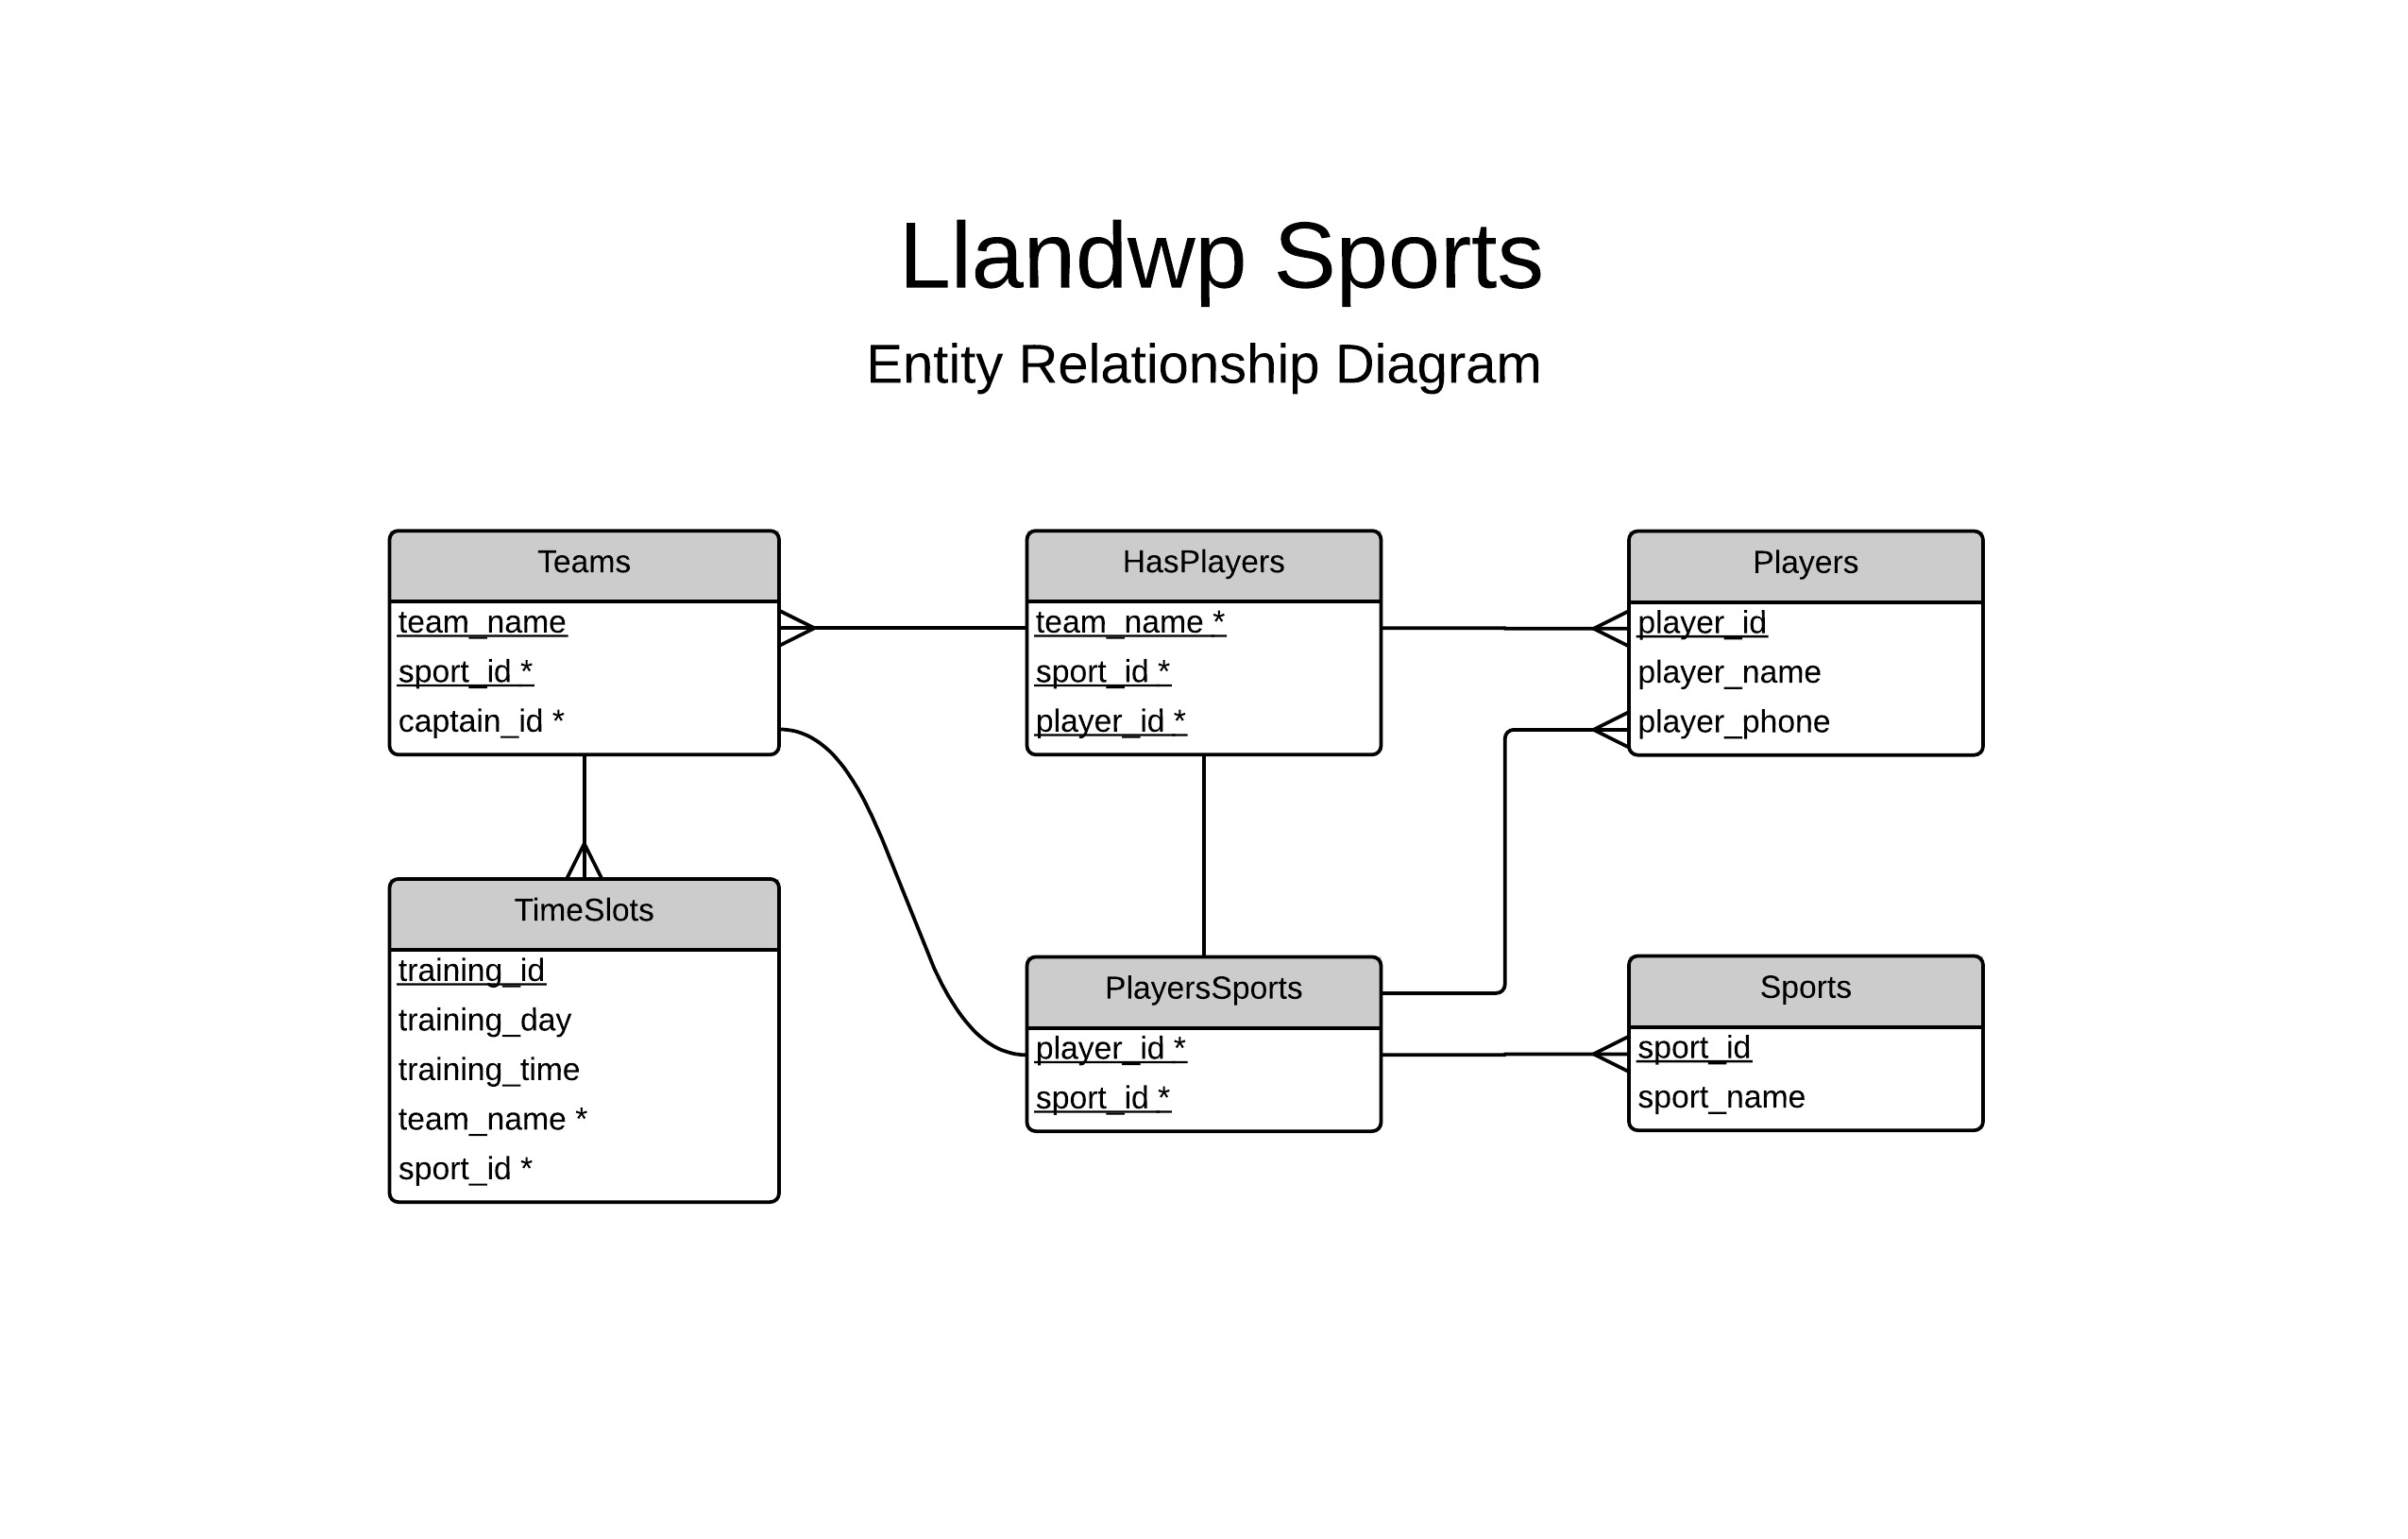
\includegraphics[width=180mm,left]{ERD.jpeg}
\end{figure}

	\section{SQL Queries}
	
	\subsection{Table Creation Queries}
	
Listed are my table creation queries that implement the schema detailed in the previous section. I used VARCHAR to hold text 20: characters for team\_name, 40 characters for player\_name and 15 characters for phone\_number seem reasonable. 
I used the SERIAL type to create auto incrementing primary keys. 
The INT type is used for non-primary key IDs (Eg. foreign keys). 
I also create my own enumerated (ENUM) type to hold a listing of the days, to ensure that only the actual days can be inputted to the database. \\ 
	\begin{lstlisting}[language=sql]
/*This is my sports table, primary key sport_id, 
  to hold a list of all sports at the club
*/
create table IF NOT EXISTS sports (
	sport_id SERIAL,
	sport_name VARCHAR(20),
	PRIMARY KEY(sport_id)
);
	
/*This is my players table, primary key player_id, 
  to hold a list of all players at the club
*/
create table IF NOT EXISTS players (
	player_id SERIAL,
	player_name VARCHAR(40),
	player_phone VARCHAR(15),
	PRIMARY KEY(player_id)
);
	
/*This is my players_sports table, primary composite key player_id,
  sport_id; foreign keys player_id, sport_id from the players and 
  sports tables. This is my linking table to establish the many-to-many
  relationship between players and sports. It assigns a sport to a player, 
  without a team. This is also where the teams table takes it's sport 
  and captain.
*/
create table IF NOT EXISTS players_sports (
    	player_id INT REFERENCES players(player_id),
    	sport_id INT REFERENCES sports(sport_id),
    	PRIMARY KEY (player_id, sport_id)
);









/*This is my teams table, primary composite key team_name, sport_id;
  foreign key sport_id, captain_id from the players_sports table. 
  This table holds all the teams at the club,  the sport it plays, 
  and it's captain
*/
create table IF NOT EXISTS teams (
	team_name VARCHAR(20),
	sport_id INT,	
	captain_id INT,
	FOREIGN KEY (sport_id, captain_id) 
		REFERENCES players_sports(sport_id, player_id),
	PRIMARY KEY (team_name, sport_id)

);
/*This is my has_players table, primary composite key team_name, sport_id,
  player_id; foreign keys team_name, sport_Id from the teams table. This is
  my linking table to establish the many-to-many relationship between teams
  and players.
*/
create table IF NOT EXISTS has_players (
	team_name VARCHAR(20),
	sport_id int,
	player_id INT REFERENCES players(player_id),
	FOREIGN KEY (team_name, sport_id) 
		REFERENCES teams(team_name, sport_id),
	FOREIGN KEY (player_id, sport_id)
    		REFERENCES players_sports(player_id, sport_id),
	PRIMARY KEY(team_name, sport_id, player_id)
);

/*This is the enumerated DAY type I created which holds all the days 
  a training_day can hold.
*/
CREATE TYPE DAY AS ENUM (
  	'Monday',
  	'Tuesday',
  	'Wednesday',
 	'Thursday',
 	'Friday',
  	'Saturday',
  	'Sunday'
);



/*This is my time_slot table, primary key training_ID; foreign keys 
  team_name,  sport_id from the teams table to establish the 
  one-to-many relationship. This table holds all the training day/time
  data for each team.
*/
create table IF NOT EXISTS time_slot (
	training_id SERIAL,
	training_day DAY,
	training_time TIME,
	team_name VARCHAR(20),
	sport_id int,	
	FOREIGN KEY (team_name, sport_id) 
		REFERENCES teams (team_name, sport_id),
	PRIMARY KEY (training_id)
);
	
	\end{lstlisting}


	\subsection{Insert Queries}
	
	\begin{lstlisting}[language=sql]
/*Insert 7 players into the players table.*/

INSERT INTO players (player_name, player_phone) 
	VALUES ('Max', '07949028660');
INSERT INTO players (player_name, player_phone) 
	VALUES ('Hannah', '07945624312');
INSERT INTO players (player_name, player_phone) 
	VALUES ('Chandlar', '07947687776');
INSERT INTO players (player_name, player_phone) 
	VALUES ('Edward', '07945432123');
INSERT INTO players (player_name, player_phone) 
	VALUES ('Liam', '07945678765');
INSERT INTO players (player_name, player_phone) 
	VALUES ('Erin', '07949996758');
INSERT INTO players (player_name, player_phone) 
	VALUES ('Ffion', '07946576566');

/*Insert 4 sports into the sports table.*/
INSERT INTO sports (sport_name) 
	VALUES ('Soccer');
INSERT INTO sports (sport_name) 
	VALUES ('Table Tennis');
INSERT INTO sports (sport_name) 
	VALUES ('Chess');
INSERT INTO sports (sport_name) 
	VALUES ('Squash');
INSERT INTO sports (sport_name) 
	VALUES ('Rugby');


/*Assign sports to players with no teams.*/
/*Max plays Soccer*/
INSERT INTO players_sports(player_id, sport_id) 
	VALUES (1, 1);
/*Max plays Table Tennis.*/
INSERT INTO players_sports(player_id, sport_id) 
	VALUES (1, 2);
/*Hannah plays Soccer.*/
INSERT INTO players_sports(player_id, sport_id) 
	VALUES (2, 1);
/*Hannah plays Squash.*/
INSERT INTO players_sports(player_id, sport_id) 
	VALUES (2, 4);
/*Chandlar plays Soccer.*/
INSERT INTO players_sports(player_id, sport_id) 
	VALUES (3, 1);
/*Chandlar plays Chess*/
INSERT INTO players_sports(player_id, sport_id) 
	VALUES (3, 3);
/*Chandlar plays Squash.*/
INSERT INTO players_sports(player_id, sport_id)
	VALUES(3, 4);
/*Edward plays Soccer.*/
INSERT INTO players_sports(player_id, sport_id) 
	VALUES (4, 1);
/*Edward plays Table Tennis.*/
INSERT INTO players_sports(player_id, sport_id) 
	VALUES (4, 2);
/*Liam plays Soccer.*/
INSERT INTO players_sports(player_id, sport_id) 
	VALUES (5, 1);
/*Liam plays Chess.*/
INSERT INTO players_sports(player_id, sport_id) 
	VALUES (5, 3);
/*Erin plays Soccer.*/
INSERT INTO players_sports(player_id, sport_id) 
	VALUES (6, 1);
/*Ffion plays Table Tennis.*/
INSERT INTO players_sports(player_id, sport_id) 
	VALUES (7, 2);
/*Ffion plays Chess.*/
INSERT INTO players_sports(player_id, sport_id) VALUES (7, 3);





/*Insert 4 teams into the teams table, assigning captains and 
  sports to each.
*/
/*Hannah is the captain of Thunderbirds; they play Soccer.*/
INSERT INTO teams (team_name, sport_id, captain_id) 
	VALUES ('Thunderbirds', 1, 2);
/*Chandlar is the captain of Flying Machine; they play Soccer.*/
INSERT INTO teams (team_name, sport_id, captain_id) 
	VALUES ('Flying Machine', 1, 3);
/*Ffion is the captain of The Tables; they play Table Tennis.*/
INSERT INTO teams (team_name, sport_id, captain_id) 
	VALUES ('The Tables', 2, 7);
/*Liam is the captain of The Chessers; they play Chess.*/
INSERT INTO teams (team_name, sport_id, captain_id)
	VALUES ('The Chessers', 3, 5);
	
/*Broken teams query to show a captain must play the sport first*/
INSERT INTO teams (team_name, sport_id, captain_id)
	VALUES ('The Chessers', 3, 5);




























/*Assign players to their teams*/
/*Max plays with Thunderbirds.*/
INSERT INTO has_players (team_name, sport_id, player_id) 
	VALUES ('Thunderbirds', 1, 1);
/*Liam plays with Thunderbirds.*/
INSERT INTO has_players (team_name, sport_id, player_id) 
	VALUES ('Thunderbirds', 1, 5);
/*Erin plays with Thunderbirds.*/
INSERT INTO has_players (team_name, sport_id, player_id) 
	VALUES ('Thunderbirds', 1, 6);
/*Edward plays with Flying Machine.*/
INSERT INTO has_players (team_name, sport_id, player_id) 
	VALUES ('Flying Machine', 1, 4);
/*Edward plays with The Tables.*/
INSERT INTO has_players (team_name, sport_id, player_id) 
	VALUES ('The Tables', 2, 4);
/*Max plays with The Tables.*/
INSERT INTO has_players (team_name, sport_id, player_id) 
	VALUES ('The Tables', 2, 1);
/*Chandlar plays with The Chessers.*/
INSERT INTO has_players (team_name, sport_id, player_id) 
	VALUES ('The Chessers', 3, 3);
/*Ffion plays with The Chessers.*/
INSERT INTO has_players (team_name, sport_id, player_id) 
	VALUES ('The Chessers', 3, 7);
	
/*Broken has_players query to prove a player must play a 
  sport before being a part of the team
  */
INSERT INTO has_players (team_name, sport_id, player_id) 
	VALUES ('The Chessers', 4, 1);

/*Assign training days and times to each team.*/
INSERT INTO time_slot (training_day, training_time, team_name, sport_id)
	VALUES ('Tuesday', '09:30', 'Thunderbirds', 1);
INSERT INTO time_slot (training_day, training_time, team_name, sport_id)
	VALUES ('Thursday', '14:30', 'Thunderbirds', 1);
INSERT INTO time_slot (training_day, training_time, team_name, sport_id)
	VALUES ('Monday', '10:00', 'Flying Machine', 1);
INSERT INTO time_slot (training_day, training_time, team_name, sport_id)
	VALUES ('Sunday', '04:00', 'The Tables', 2);
INSERT INTO time_slot (training_day, training_time, team_name, sport_id)
	VALUES ('Monday', '12:00', 'The Tables', 2);
INSERT INTO time_slot (training_day, training_time, team_name, sport_id)
	VALUES ('Monday', '14:00', 'The Tables', 2);
INSERT INTO time_slot (training_day, training_time, team_name, sport_id)
	VALUES ('Wednesday', '16:00', 'The Chessers', 3);

/*Broken time_slot query to prove ENUM works*/
INSERT INTO time_slot (training_day, training_time, team_name, sport_id)
	VALUES ('Fednesdays', '16:00', 'The Chessers', 3);
	
	\end{lstlisting}
	\newpage
	\subsection{Select Queries}
	
	\subsubsection{List all players for a given team}
	\begin{lstlisting}[language=sql]
	
/*List all players on the Thunderbirds team.
  Should be Max, Liam, Erin.
*/
SELECT players.player_name, players.player_phone FROM has_players 
	JOIN players ON has_players.player_id = players.player_id 
	WHERE has_players.team_name = 'Thunderbirds' 
	AND has_players.sport_id = 1;

/*List all players on the Flying Machine team.
  Should be Edward.
*/
SELECT players.player_name, players.player_phone FROM has_players 
	JOIN players on has_players.player_id = players.player_id
	WHERE has_players.team_name = 'Flying Machine' 
	AND has_players.sport_id = 1;

/*List all players on The Tables team.
  Should be Max, Edward.
*/
SELECT players.player_name, players.player_phone FROM has_players 
	JOIN players ON has_players.player_id = players.player_id
	WHERE has_players.team_name = 'The Tables' 
	AND has_players.sport_id = 2;

/*List all players on The Chessers team.
  Should be Chandlar, Ffion.
*/
SELECT players.player_name, players.player_phone FROM has_players 
	JOIN players ON has_players.player_id = players.player_id
	WHERE has_players.team_name = 'The Chessers' 
	AND has_players.sport_id = 3;

\end{lstlisting}
\newpage
	\subsubsection{List all players for a given sport}
	\begin{lstlisting}[language=sql]

/*List all players who play Soccer.
  Should be Max, Hannah, Chandlar, Edward, Liam, Erin
*/
SELECT sports.sport_name, players.player_name FROM players_sports
	JOIN players ON players_sports.player_id = players.player_id
	JOIN sports ON  sports.sport_id = players_sports.sport_id
	WHERE sports.sport_name  = 'Soccer';

/*List all players who play Table Tennis.
  Should be Max, Edward, Ffion.
*/
SELECT sports.sport_name, players.player_name FROM players_sports
	JOIN players ON players_sports.player_id = players.player_id
	JOIN sports ON  sports.sport_id = players_sports.sport_id
	WHERE sports.sport_name  = 'Table Tennis';

/*List all players who play Chess.
  Should be Chandlar, Liam, Ffion.
*/
SELECT sports.sport_name, players.player_name FROM players_sports
	JOIN players ON players_sports.player_id = players.player_id
	JOIN sports ON  sports.sport_id = players_sports.sport_id
	WHERE sports.sport_name  = 'Chess';

/*List all players who play Squash.
  Should be Hannah.
*/
SELECT sports.sport_name, players.player_name FROM players_sports
	JOIN players ON players_sports.player_id = players.player_id
	JOIN sports ON  sports.sport_id = players_sports.sport_id
	WHERE sports.sport_name  = 'Squash';
	
	\end{lstlisting}

	\subsubsection{List all sports with no assigned teams}
	\begin{lstlisting}[language=sql]
SELECT sports.sport_name FROM sports
	LEFT JOIN teams ON teams.sport_id = sports.sport_id
	WHERE teams.sport_id IS NULL;
	\end{lstlisting}

	\subsubsection{List all sports with no assigned players}
	\begin{lstlisting}[language=sql]
SELECT sports.sport_name FROM sports 
	LEFT JOIN players_sports ON players_sports.sport_id = sports.sport_id
	WHERE players_sports.sport_id IS NULL;
	\end{lstlisting}

\section{Screenshots using PHPPGAdmin}

\begin{figure}[ht!]
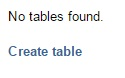
\includegraphics[center]{NoTables.jpg}
\caption{Empty database.}
\end{figure}

\begin{figure}[ht!]
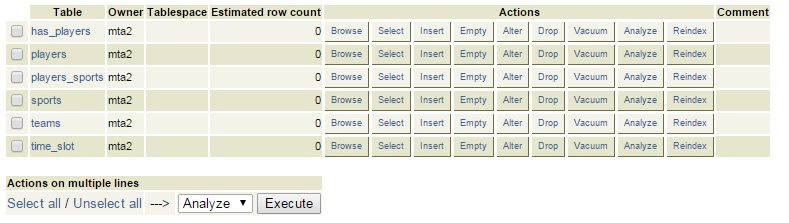
\includegraphics[center]{CreatedTables.png}
 \caption{Used creation queries listed above.}
\end{figure}

\begin{figure}[ht!]
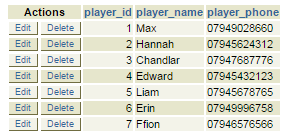
\includegraphics[center]{PlayersTable.png}
 \caption{Inserted players.}
\end{figure}

\begin{figure}[ht!]
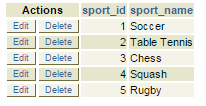
\includegraphics[center]{SportsTable.png}
 \caption{Inserted sports.}
\end{figure}

\begin{figure}[ht!]
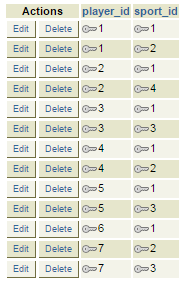
\includegraphics[center]{PlayersSports.png}
 \caption{Inserted player-sports relations.}
\end{figure}

\begin{figure}[ht!]
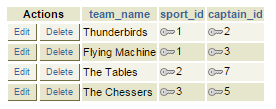
\includegraphics[center]{Teams.png}
 \caption{Inserted teams with captains.}
\end{figure}

\begin{figure}[ht!]
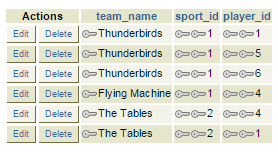
\includegraphics[center]{HasPlayers.png}
 \caption{Inserted teams-players relations.}
\end{figure}

\begin{figure}[ht!]
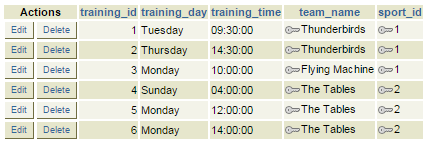
\includegraphics[center]{Timeslot.png}
 \caption{Inserted timeslots for teams.}
\end{figure}

\begin{figure}[ht!]
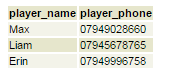
\includegraphics[center]{Thunderbirds.png}
 \caption{Players who play for Thunderbirds.}
\end{figure}

\begin{figure}[ht!]
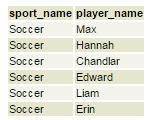
\includegraphics[center]{Soccer.png}
 \caption{Players who play Soccer.}
\end{figure}

\begin{figure}[ht!]
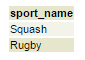
\includegraphics[center]{NoTeams.png}
 \caption{Sports with no teams}
\end{figure}

\begin{figure}[ht!]
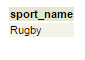
\includegraphics[center]{NoPlayers.png}
 \caption{Sports with no players.}
\end{figure}

\begin{figure}[ht!]
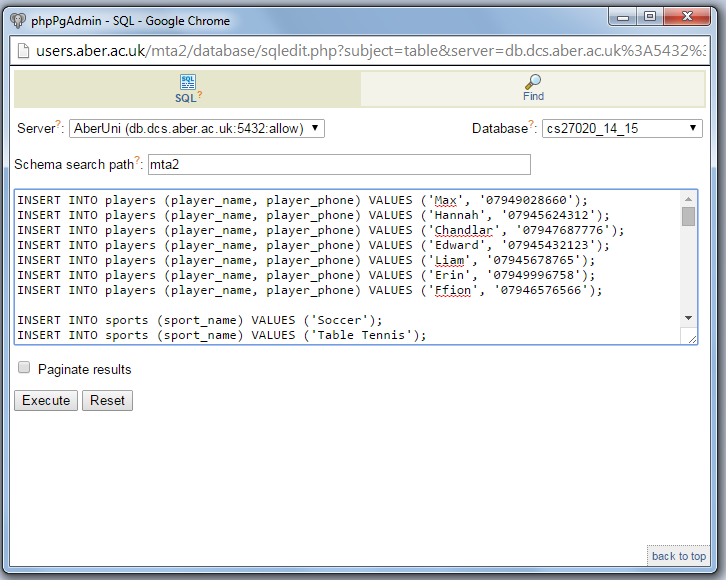
\includegraphics[center]{QueryExecuter.png}
 \caption{How I executed my queries, not using provided tools.}
\end{figure}

\end{document}
